\documentclass[USenglish,oneside,twocolumn]{article}

\usepackage[utf8]{inputenc}%(only for the pdftex engine)
%\RequirePackage[no-math]{fontspec}%(only for the luatex or the xetex engine)
\usepackage[big]{dgruyter_NEW}

\DOI{foobar}

\cclogo{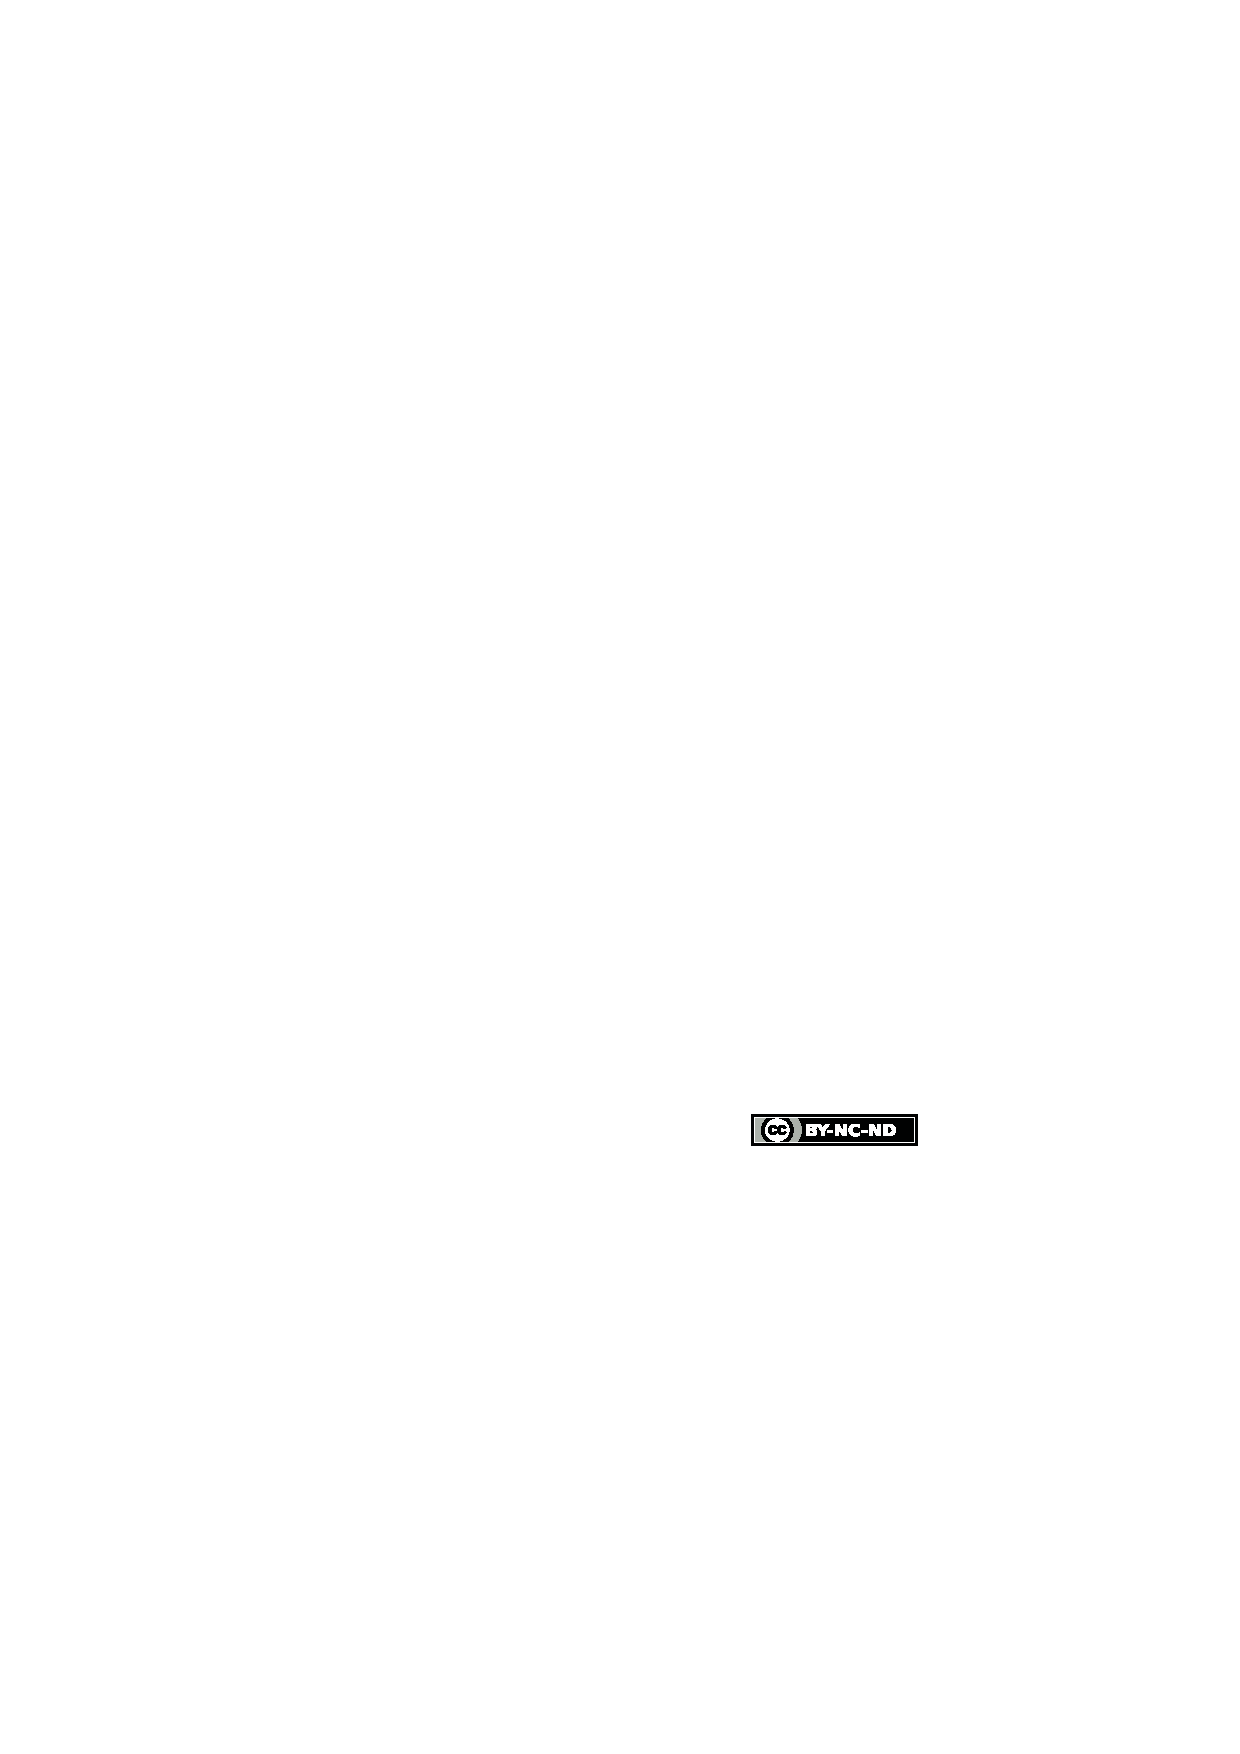
\includegraphics{by-nc-nd.pdf}}

% Related work comparison table
\usepackage{amsmath,wasysym} % \CIRCLE, \Circle
\usepackage{multirow} % \multirow
\usepackage{times} % font in table header


\begin{document}


  \author[1]{Anthony P. Machado}

  \author[2]{Gaby G. Dagher}

  \affil[1]{Boise State University, E-mail: anthonymachado@u.boisestate.edu}

  \affil[2]{Boise State University, E-mail: gabydagher@boisestate.edu}

  \title{\huge Hiding Data in Cellular DNA: Contextualizing Diverse Encoding Schemes}

  \runningtitle{Hiding Data in Cellular DNA}

  %\subtitle{...}

  \begin{abstract}
{DNA, the macromolecule used by organisms to store and transmit genomic data, has attracted the attention of privacy researchers as a channel for secure data transfer. DNA's small size and abundance in nature makes it an ideal steganographic medium for hiding messages. Already, artificially synthesized DNA has been used to store text, audio, and images. Encoded cellular DNA is not far behind, with much research being done on ways to safely embed data without harming the cell. \\
In this survey we provide the first systematic comparison of cellular encoding schemes proposed in the literature. Different DNA regions in the cell have their own unique bio-restrictions that must be satisfied for DNA storage. Drawing from a wide array of schemes, we compare the novel techniques used to meet these bio-restrictions. This contextualization of the research creates a bigger picture that can help guide the design of future schemes. We also survey the compression methods and error detection techniques used by the encoding schemes, and their effect on error rate and bits-per-base density. Finally, we propose future directions for research in untapped cellular regions such as mitochondrial DNA and we offer novel insights into the potential for epigenetic encoding with methylation and histones.}
\end{abstract}

  \keywords{keywords, keywords}
%  \classification[PACS]{}
 % \communicated{...}
 % \dedication{...}
 % \test

  \journalname{Proceedings on Privacy Enhancing Technologies}
\DOI{Editor to enter DOI}
  \startpage{1}
  \received{..}
  \revised{..}
  \accepted{..}

  \journalyear{2017}
  \journalvolume{2017}
  \journalissue{3}


\maketitle
\section{Introduction}

Biosteganography is an emerging field in privacy research that combines techniques from genetic engineering, bioinformatics, cryptography and forensics to secretly transfer data within a living cell's DNA~\cite{B2016JOB}. Data ranging from simple text messages to audio recordings and color images can be inserted into cellular DNA. Because DNA is information dense and occurs abundantly in nature, it makes an ideal medium for sending messages secretly. Basic steganographic principles dictate that if an attacker doesn’t know where to find a confidential message in the first place, the message is far more secure.

Traditional digital storage systems such as hard drives and SD cards have detectable emanations, which makes them vulnerable to side attacks~\cite{T2008TOIAS}. Modified DNA, however, has no measurable emanations. If an agent needed to carry a hidden message through a tight security checkpoint, any form of electronic storage could be easily detected, while physical recordings like paper or tape could be visibly located by the security guard. A DNA encoded message, however, located in the cells of the agent's thumb, or in bacteria under the agent's nail, could be brought through without detection. The receiver of the message, of course, would need to know how to decode the data, and have the lab equipment to amplify and sequence the DNA.

In this survey,

- storage capacity
- watermarking
- in this work


\section{Background}

\subsection{DNA}

Every living cell contains DNA molecules encoded with instructions for making the proteins necessary for the cell to function. DNA takes the form of a double helix made of two antiparallel strands. Each strand is composed of a sequence of 4 nucleotides: adenine (A), guanine (G), cytosine (C), and thymine (T). The purines adenine and guanine, and the pyrimidines cytosine and thymine hydrogen bond with each other across the double helix. Every three nucleotides forms a codon that the cell reads and processes to create an amino acid, the building block of a protein~\cite{WC1953N}.

There are only 20 amino acids, despite the fact that $4^3$ = 64 possible codon variations exist. This is because many amino acids have up to five redundant codons. Also, three codons are used specifically as stop signals to indicate the end of a protein chain. The redundancy in codon to amino acid mapping is called codon degeneracy~\cite{WBBGLL2008}. Codon degeneracy gives an evolutionary advantage to the cell by allowing certain mutations to occur in a codon while preserving the codon’s functionality.

\subsection{Artificial DNA Encoding}

 DNA was first encoded with a secret message in 1999 by Clelland et al~\cite{CRB1999N}. Inspired by the tiny, concealed “microdot” messages used in World War II, artificial DNA strands were constructed using a simple substitution cipher, then mixed with human DNA and pipetted onto a printed period on filter paper. The encoded DNA was later recovered from the dot and sequenced to successfully read the secret message: “JUNE 6 INVASION: NORMANDY”.

\section{Bio-Restrictions}

Cellular DNA encoding must not harm the carrier organism, either by removing cellular functionality or adding mutative behavior. To avoid this, encoding schemes must ensure that modified DNA strands remain biologically equivalent to their wild-type form. This section defines the bio-restrictions that exist for two distinct areas of cellular DNA, protein coding DNA (pcDNA) and noncoding DNA (ncDNA). As our knowledge of genetics continues to expand, more particular restrictions may become known.

\subsection{pcDNA Constraints}

The protein coding region of DNA contains the codons that are translated to amino acids, which are then concatenated into proteins. Any data insertions in this area must meet the following constraints.

\textit{Protein Preservation} The structure of the protein coded by the region must remain unchanged.

\textit{Codon Bias Preservation}


\subsection{ncDNA Constraints}

The noncoding region of DNA is often called "junk DNA" for its apparent lack of use in the cell. Because these regions appear to be non-functional, data can be embedded into these regions if the following constraints are met.

\textit{Truly nonfunctional region.} When ncDNA was first discovered it was assumed to have no role in cell functionality, but recent studies have shown that up to 80\% of ncDNA may have biochemical functions in the cell, despite not coding for proteins~\cite{EPC2012N}. Therefore, it is first imperative that the individual who wishes to insert a message into ncDNA verify that they are encoding their message in the 20\% that has no biochemical use.

\textit{No start codons.} When a cell's genetic machinery locates a start codon, it can begin the transcription process. To prevent unwanted transcription from happening in ncDNA with embedded data, it is important to make sure the encoded nucleotides to not create a start codon. When a DNA string is being transcribed, three-nucleotide codons can be read in six different reading frames. Therefore, there should not be a start codon in any of the six frames. The most common start codon is AUG, though some alternative start codons can also exist, particularly in bacteria~\cite{B1997S}. If a cell contains alternative start codons, the encoding scheme should avoid all of them.

\textit{No homopolymers.} A DNA homopolymer is a region where the same nucleotide is repeated multiple times. Too many repeats can cause errors during DNA replication through polymerase slippage~\cite{VCE2001TEJ}. These replication errors could quickly distort the inserted message and possible damage the cell after a few generations. For this reason any ncDNA encoding scheme should not include homopolymers greater than length 3.


\section{Encoding Schemes}

Encoding schemes for cellular DNA can involve several components:

\begin{enumerate}
\item Encryption algorithm
\item Mapping table
\item Compression
\item Error correction
\item Fake data embedding
\end{enumerate}

The following encoding schemes use some or all of these elements in their design.

\subsection{pcDNA Encoding}

Shimanovsky et al~\cite{SFHC2003BL} were the first to propose using codon degeneracy to encode data in pcDNA. By switching codons between their redundant forms with the modification of one nucleotide, data could be inserted without altering protein translation. Arita and Ohashi ~\cite{AY2004BP} were the first to implement this scheme in a living cell. They did this using site-directed mutagenesis of wobble codons in the \textit{ftsZ} gene of \textit{Bacillus subtilis}. The university name "KEIO" was inserted by modifying the redundant nucleotides of the codons downstream of the \textit{ftsZ} start codon. An unmodified codon represented value 0 while a codon with a wobble nucleotide changed to any of its non-wild type redundant forms represented value 1. Messages were translated using a 6-bit mapping table, with the first 5 bits corresponding to an English alphabet letter or basic punctuation, and the last used as a parity bit for error correction.



\begin{center}
 \begin{tabular}{||c || c c c c||}
 \hline
  & U & C & A & G \\ [0.5ex]
 \hline\hline
 U & 6 & 87837 & 787 \\
 \hline
 C & 7 & 78 & 5415 \\
 \hline
 A & 545 & 778 & 7507 \\
 \hline
 G & 545 & 18744 & 7560 \\
 \hline
 5 & 88 & 788 & 6344 \\ [1ex]
 \hline
\end{tabular}
\end{center}

\subsection{ncDNA Encoding}

\subsection{Plasmid Encoding}

\section{Compression and Error Correction}

Smith et al~\cite{SFHC2003BL} were the first to suggest a data compression technique in DNA encoding, specifically the Huffman Code. The Huffman Code is a form of lossless data compression that forms a symbol table using fewer bits to encode more common characters~\cite{H1952POTIRE}. Smith et al created a Huffman Code table mapping letters of the alphabet to nucleotide strings, where the most common English letter 'e' was mapped to the nucleotide string "T", and the least common english letter 'z' was mapped to a longer nucleotide string "CCCTG". This achieved an average encoding length of 2.2 bases per letter. The mapping is unambiguous, making only one possible interpretation of each message.

\begin{table*}[!t]
    \centering
    \caption{Comparative evaluation of encoding schemes}
    \label{tbl:related_work}
    \scalebox{0.7}{
        \begin{tabular}{|p{5.7cm}|p{1.0cm}|p{0.7cm}|p{1.4cm}|p{1.1cm}|p{1.4cm}|p{1.1cm}|p{0.7cm}|p{0.8cm}|p{0.6cm}|p{0.8cm}|p{0.6cm}|p{1.1cm}|p{1.5cm}|}
            \hline
            \multirow{2}{*}{\vspace{-2cm}\textbf{Approach}} & \multicolumn{2}{|c|}{\textbf{Data Type}} & \multicolumn{4}{|c|}{\vspace{0cm}\textbf{Privacy-Preserving Domain}} & \multicolumn{5}{|c|}{\textbf{Hosting Environment}} & \multicolumn{2}{|c|}{\textbf{Security}} \tabularnewline
             \cline{2-14}
             & \vspace{0cm}\textbf{Set-Valued} & \vspace{0cm}\textbf{Other} & \multicolumn{2}{|c|}{\vspace{-.2cm}\textbf{Non-Interactive}} & \multicolumn{2}{|c|}{\vspace{0cm}\textbf{Interactive}} & \vspace{0cm}\textbf{Single} & \multicolumn{2}{|c|}{\vspace{-0.2cm}\textbf{Two}}& \multicolumn{2}{|c|}{\vspace{0cm}\textbf{Multiple}} & \vspace{0cm}\textbf{Threat Model $^\dagger$} & \vspace{0cm}\textbf{Public \newline Verifiability} \tabularnewline
             \cline{4-7}
             \cline{9-12}
             &  &  & \vspace{0cm}\textbf{Differential Privacy} & \vspace{0cm}\textbf{Syntactic Privacy} & \vspace{0cm}\textbf{Differential Privacy} & \vspace{0cm}\textbf{Syntactic Privacy}&  & \vspace{0cm}\textbf{Horiz.} & \vspace{0cm}\textbf{Vert.} & \vspace{0cm}\textbf{Horiz.} & \vspace{0cm}\textbf{Vert.}  &  & \tabularnewline
            \cline{1-14}
            \hline\hline
            Terrovitis \emph{et al.}, He and Naughton  & \centering{$\CIRCLE$} &  &  & \centering{$\CIRCLE$} &  &  & \centering{$\CIRCLE$} &  &  &  &  &  &  \tabularnewline
            \hline
            Chen \emph{et al.} &  \centering{$\CIRCLE$} &  &  \centering{$\CIRCLE$} &  &  &  & \centering{$\CIRCLE$} &  &  &  &  &  &  \tabularnewline
            \hline
            Jiang and Clifton &  &  \centering{$\CIRCLE$} &  & \centering{$\CIRCLE$} &  &  &  &  & \centering{$\CIRCLE$} &  &  & \centering{$\Circle$} &  \tabularnewline
            \hline
            Jurczyk and Xiong &  &  \centering{$\CIRCLE$} &  & \centering{$\CIRCLE$} &  &  &  &  &  & \centering{$\CIRCLE$} &  & \centering{$\Circle$} &  \tabularnewline
            \hline
            Alhadidi \emph{et al.} &  &  \centering{$\CIRCLE$} & \centering{$\CIRCLE$} &  &  &  &  & \centering{$\CIRCLE$} &  &  &  & \centering{$\Circle$} &  \tabularnewline
            \hline
            Mohammed \emph{et al.} (DistDiffGen) &  & \centering{$\CIRCLE$} & \centering{$\CIRCLE$} &  &  &  &  &  & \centering{$\CIRCLE$} &  &  & \centering{$\Circle$} &  \tabularnewline
            \hline
            Mohammed \emph{et al.} (TIPS) &  & \centering{$\CIRCLE$} &  & \centering{$\CIRCLE$} &  &  &  &  & \centering{$\CIRCLE$} &  &  & \centering{$\CIRCLE$} &  \tabularnewline
            \hline
            Bhaskar \emph{et al.}, Li \emph{et al.} & \centering{$\CIRCLE$} &  &  &  & \centering{$\CIRCLE$} &  & \centering{$\CIRCLE$} &  &  &  &  &  &  \tabularnewline
            \hline
            Wong \emph{et al.}  & \centering{$\CIRCLE$} &  &  &  &  &  & \centering{$\CIRCLE$} &  &  &  &  & \centering{$\Circle$} &  \tabularnewline
            \hline
            Giannotti \emph{et al.} & \centering{$\CIRCLE$} &  &  &  &  & \centering{$\CIRCLE$} & \centering{$\CIRCLE$} &  &  &  &  & \centering{$\Circle$} &  \tabularnewline
            \hline
            Kantarcioglu and Clifton & \centering{$\CIRCLE$} &  &  &  &  &  &  &  &  & \centering{$\CIRCLE$} &  & \centering{$\Circle$} &  \tabularnewline
            \hline
            Zhang \emph{et al.} & \centering{$\CIRCLE$} &  &  &  &  &  &  & \centering{$\CIRCLE$} &  &  &  & \centering{$\Circle$} &  \tabularnewline
            \hline
            Wahab \emph{et al.} & \centering{$\CIRCLE$} &  &  &  & \centering{$\CIRCLE$} &  &  & \centering{$\CIRCLE$} &  & \centering{$\CIRCLE$} &  & \centering{$\Circle$} &  \tabularnewline
            \hline
            Dwork \emph{et al.} &  & \centering{$\CIRCLE$} &  &  & \centering{$\CIRCLE$} &  &  &  &  & \centering{$\CIRCLE$} &  & \centering{$\CIRCLE$} &  \tabularnewline
            \hline
            Narayan and Haeberlen &  & \centering{$\CIRCLE$} &  &  & \centering{$\CIRCLE$} &  &  & \centering{$\CIRCLE$} & & \centering{$\CIRCLE$} &  & \centering{$\Circle$} &  \tabularnewline
            \hline\hline
            Our proposed solution &  \centering{$\CIRCLE$} &  &  \centering{$\CIRCLE$} &  &  &  &  & \centering{$\CIRCLE$} & \centering{$\CIRCLE$} & \centering{$\CIRCLE$} & \centering{$\CIRCLE$} & \centering{$\CIRCLE$} & \centering{$\CIRCLE$} \tabularnewline
            \hline
        \end{tabular}
    }
    \vspace{0.01cm}
    \newline
    $\dagger$
    \fontsize{7pt}{12pt}\selectfont
    \raggedright In this column, $\Circle$ denotes semi-honest threat model whereas $\CIRCLE$ denotes malicious threat model.
\end{table*}

\section{Future Directions}

\section{Conclusions}

\bibliographystyle{IEEEtran}
\bibliography{References}

\end{document}



\end{document}
